\section{Training Pipeline}
\label{sec:training_pipeline}

\paragraph{Action-modality training.}

Following the notation in the main manuscript, we denote the discretized instruction and observations as $l$, and apply noising and prediction only to the action modality. 
As shown in \Cref{alg:action_dfm_training},
let $x_1=[x_1^1,\ldots,x_1^D]$ be the clean action token sequence. At each training iteration, we sample $t\sim\mathcal{U}(0,1)$, draw corrupted action tokens $x_t\sim p_t(\cdot\mid x_1)$ from the prescribed probability path, and feed $(x_t, l)$ into the predictor to obtain per-position distributions $p_{1|t}^{\theta}(\cdot\mid x_t, l)$. The model refines all action tokens in parallel.

The training objective follows the same definitions in the main manuscript. Depending on the velocity modeling variant, we optimize either $\mathcal{L}_{\text{ce}}$ or $\mathcal{L}_{\text{head}}$.
% ; optionally, we use a weighted joint objective $\mathcal{L}_{\text{train}}=\mathcal{L}_{\text{ce}}+\mu\mathcal{L}_{\text{head}}$.

\begin{algorithm}[t]
\caption{Action-Modality DFM Training}
\label{alg:action_dfm_training}
\begin{algorithmic}[1]
\REQUIRE Predictor $p_\theta$, learning rate $\eta$, optional weight $\mu$
\REPEAT
    \STATE Sample $(l,x_1)\sim p_{\text{data}}$
    \STATE Sample $t\sim\mathcal{U}(0,1)$
    \STATE Sample $x_t\sim p_t(\cdot\mid x_1)$
    \STATE Choose $\mathcal{L}_{\text{train}}\in\{\mathcal{L}_{\text{ce}},\mathcal{L}_{\text{head}}\}$
    \STATE Compute $\mathcal{L}_{\text{train}}$ from $(x_t,l)$ and $x_1$
    \STATE $\theta\leftarrow\theta-\eta\nabla_\theta\mathcal{L}_{\text{train}}$
\UNTIL{converged}
\STATE \textbf{return} trained predictor $p_\theta$
\end{algorithmic}
\end{algorithm}

\section{Visualization of Refinement Process}
\label{sec:space_visualization}

To provide intuition for the action-embedding-guided velocity modeling in the main manuscript, \Cref{fig:space} visualizes a token refinement trajectory in the embedding space at three representative times ($t=0$, $t=0.5$, and $t=1$). The hollow blue circles denote candidate token IDs, the red point denotes the predicted clean token $x_1^{\mathrm{pred}}$, and $x_t$ denotes the current token state.

At each step, the transition rate favors destinations that are closer to $x_1^{\mathrm{pred}}$ than the current token. As a result, tokens within the jumpable range can be selected, and candidates nearer to $x_1^{\mathrm{pred}}$ receive higher jump probability (deeper red). As refinement proceeds, $x_t$ moves toward $x_1^{\mathrm{pred}}$, the feasible jump set becomes progressively smaller, and updates become increasingly local. This behavior illustrates how DFM-VLA balances early exploration with late-stage stabilization during iterative action refinement.

\begin{figure}[t]  
    \centering
    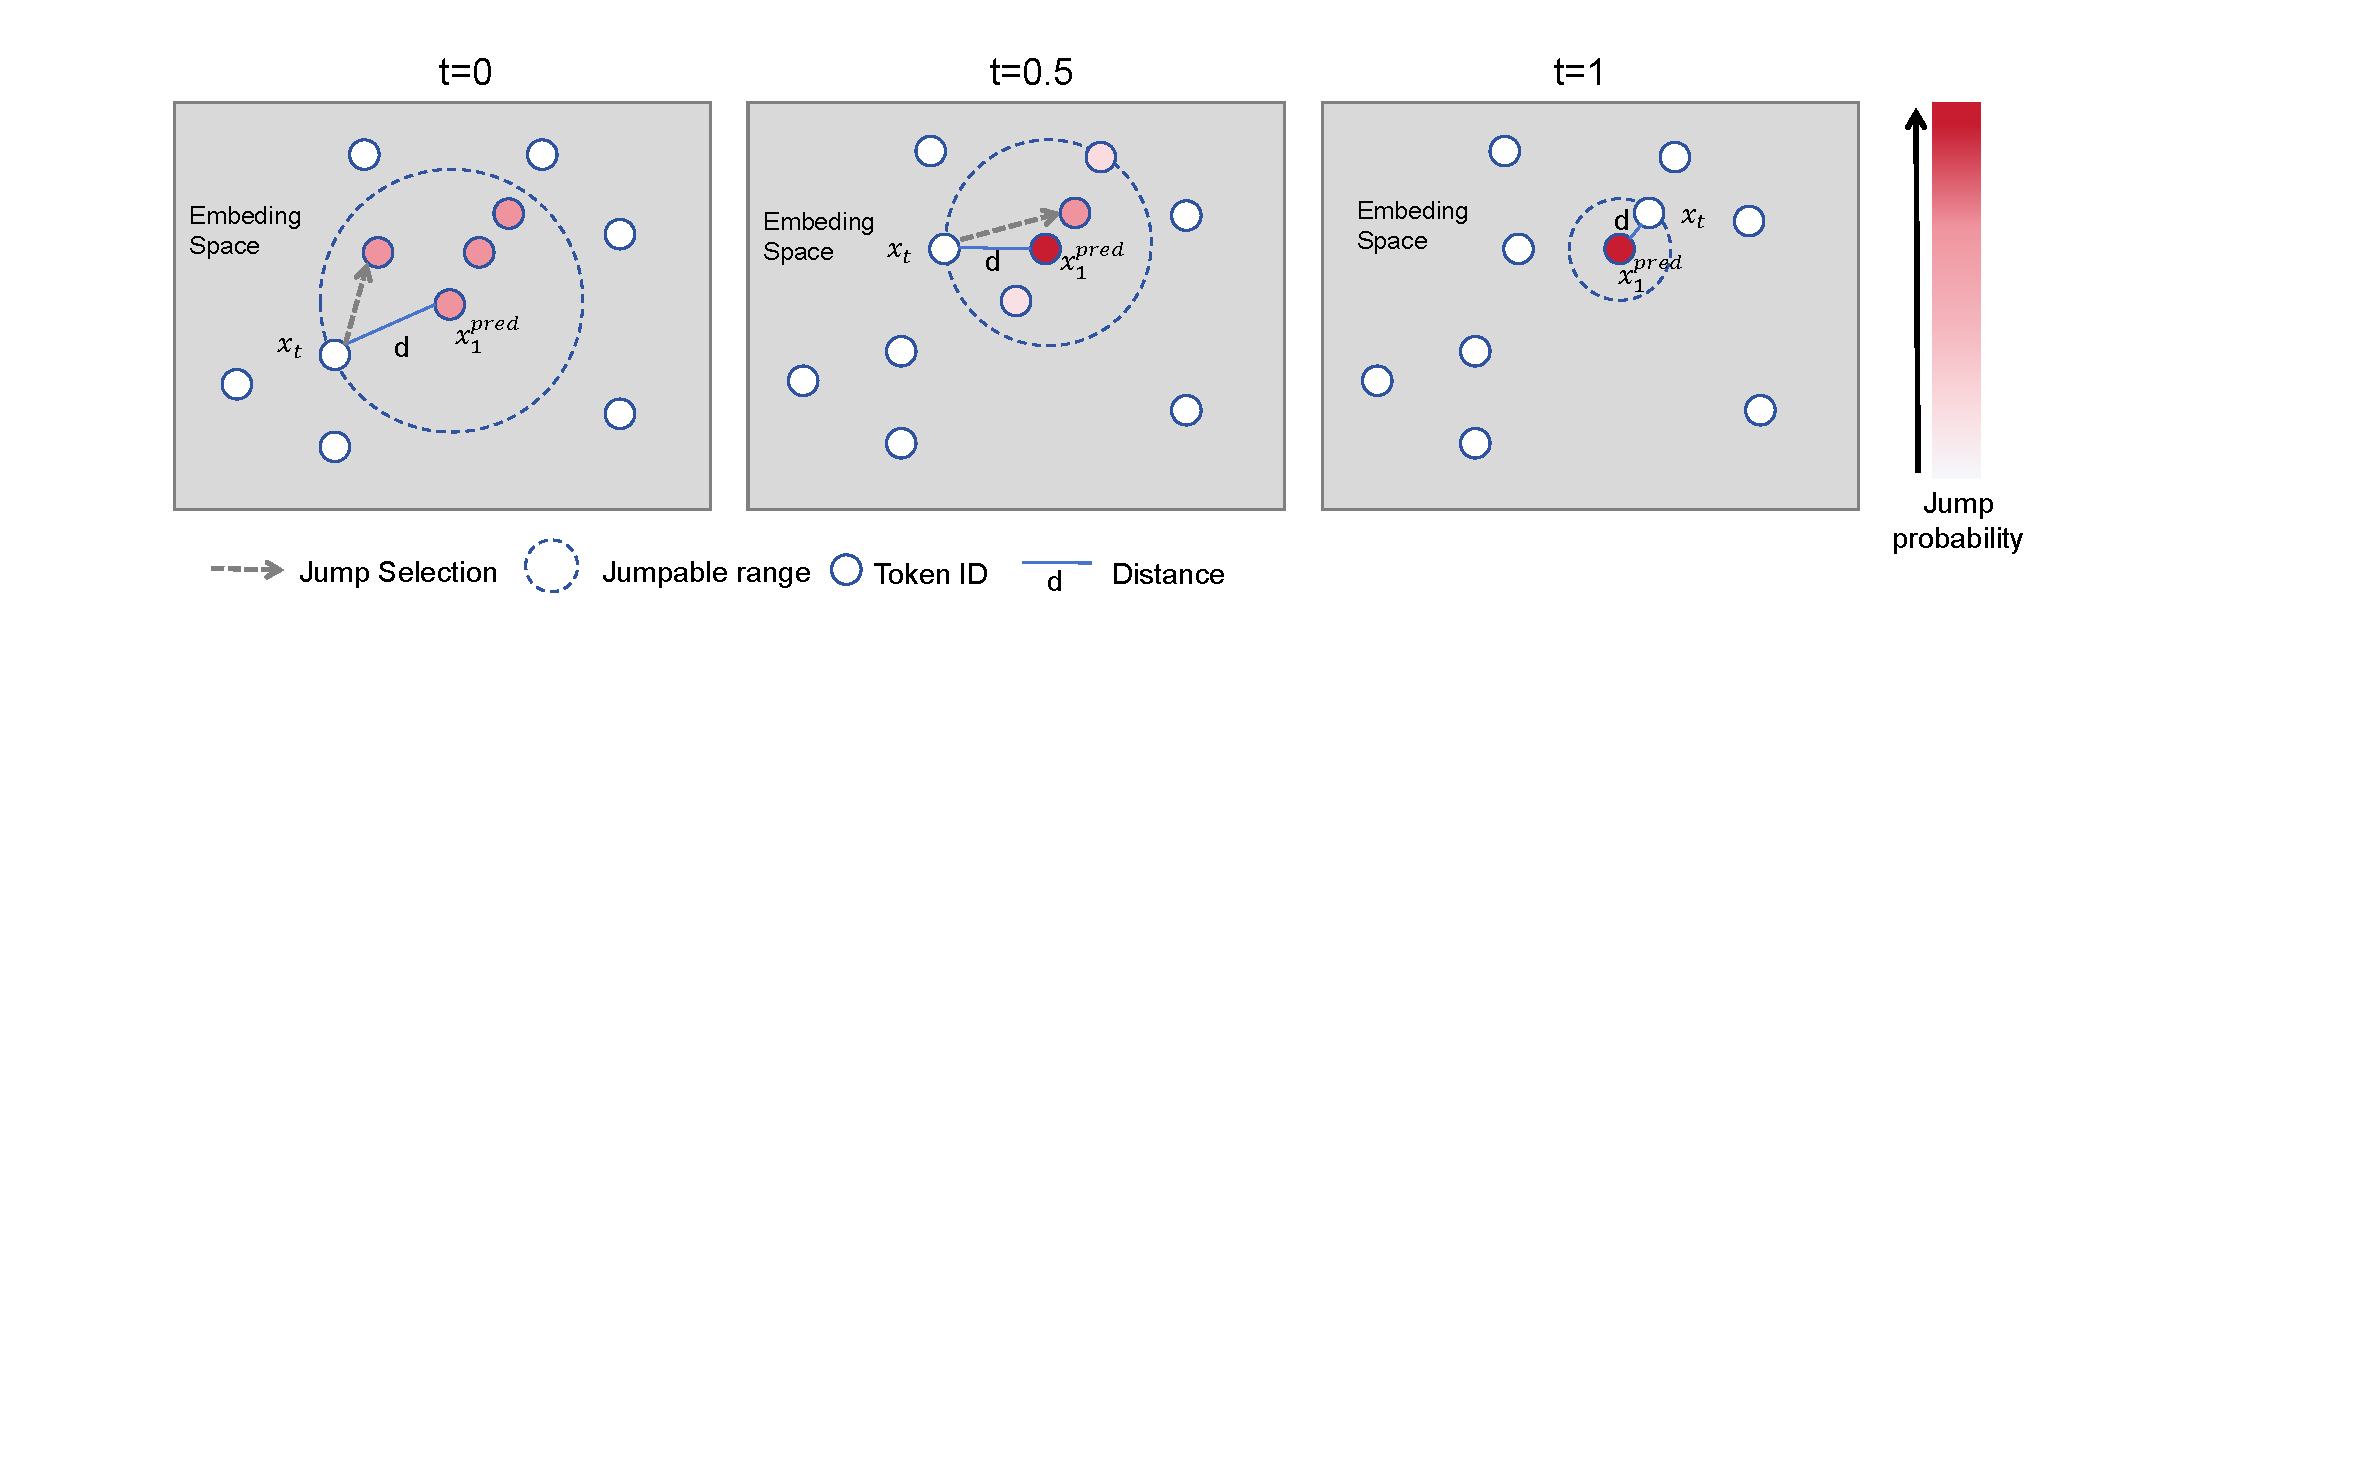
\includegraphics[width=0.98\linewidth]{figure/space.pdf} 
    \caption{Embedding-space view of iterative refinement. From $t=0$ to $t=1$, the current token $x_t$ progressively moves toward $x_1^{\mathrm{pred}}$, while transition probabilities increasingly concentrate around the target.}
    \label{fig:space} 
\end{figure}

\section{Implementation Hyperparameters}
\label{sec:implementation_hparams}

\Cref{tab:impl_hparams} summarizes the launch and training hyperparameters used in our implementation.

\begin{table}[t]
\centering
\small
\caption{Implementation hyperparameters for training.}
\label{tab:impl_hparams}
\begin{tabular}{p{0.45\linewidth}p{0.47\linewidth}}
\toprule
\textbf{Parameter} & \textbf{Value} \\
\midrule
\texttt{nproc\_per\_node} & \texttt{8} \\
\texttt{nnodes} & \texttt{1} \\
% \texttt{node\_rank} & \texttt{\$\{RANK\}} \\
% \texttt{master\_addr} & \texttt{\$\{MASTER\_ADDR\}} \\
% \texttt{master\_port} & \texttt{\$\{MASTER\_PORT\}} \\
% \texttt{train script} & \texttt{train/train\_moe.py} \\
% \texttt{model\_name\_or\_path} & \texttt{\$\{MODEL\_PATH\}} \\
% \texttt{model\_config\_path} & \texttt{configs/moe\_fast\_video.json} \\
% \texttt{deepspeed} & \texttt{scripts/sft/zero3.json} \\
% \texttt{output\_dir} & \texttt{logs/libero/\$\{EXP\_NAME\}} \\
% \texttt{data\_path} & \texttt{\$\{DATAPATH\}} \\
% \texttt{action\_tokenizer\_path} & \texttt{\$\{ACTION\_TOKENIZER\_PATH\}} \\
\texttt{learning\_rate} & \texttt{8e-5} \\
\texttt{min\_learning\_rate} & \texttt{5e-6} \\
\texttt{lr\_scheduler\_type} & \texttt{cosine\_with\_min\_lr} \\
\texttt{warmup\_steps} & \texttt{50} \\
\texttt{weight\_decay} & \texttt{0.1} \\
\texttt{max\_grad\_norm} & \texttt{5.0} \\
\texttt{adam\_beta1} / \texttt{adam\_beta2} & \texttt{0.9} / \texttt{0.95} \\
\texttt{adam\_epsilon} & \texttt{1e-6} \\
\texttt{bf16} / \texttt{tf32} & \texttt{True} / \texttt{True} \\
\texttt{max\_steps} & \texttt{16000} \\
% \texttt{per\_device\_train\_batch\_size} & \texttt{6} \\
\texttt{gradient\_accumulation\_steps} & \texttt{4} \\
\texttt{effective global batch size} & \texttt{8 * NGPUS * 4} \\
% \texttt{dataloader\_num\_workers} & \texttt{16} \\
% \texttt{gradient\_checkpointing} & \texttt{True} \\
% \texttt{frames} / \texttt{action\_frames} & \texttt{1} / \texttt{10} \\
% \texttt{max\_position\_embeddings} & \texttt{1370} \\
% \texttt{null\_prompt\_prob} & \texttt{0.15} \\
% \texttt{seed} & \texttt{42} \\
% \texttt{logging\_steps} & \texttt{20} \\
% \texttt{save\_strategy} / \texttt{save\_steps} & \texttt{steps} / \texttt{6000} \\
% \texttt{eval\_strategy} & \texttt{no} \\
% \texttt{apply\_loss\_on\_only\_vision} & \texttt{False} \\
% \texttt{apply\_loss\_on\_only\_action} & \texttt{True} \\
% \texttt{actions} / \texttt{actions\_format} & \texttt{True} / \texttt{fast} \\
% \texttt{use\_gripper} & \texttt{True} \\
% \texttt{video\_format} & \texttt{interleave} \\
\bottomrule
\end{tabular}
\end{table}
% \newpage
